% sage_latex_guidelines.tex V1.20, 14 January 2017

\documentclass[Afour,sageh,times,square,numbers]{sagej}

\usepackage{moreverb,url}
\usepackage[colorlinks,bookmarksopen,bookmarksnumbered,citecolor=red,urlcolor=red]{hyperref}
\usepackage{rotating}
\usepackage{multirow}
\usepackage{tabularx}
\usepackage{graphicx}
\usepackage{adjustbox}

\newcommand\BibTeX{{\rmfamily B\kern-.05em \textsc{i\kern-.025em b}\kern-.08em
T\kern-.1667em\lower.7ex\hbox{E}\kern-.125emX}}
\newcolumntype{C}{>{\centering\arraybackslash}p{2cm}}

%\usepackage{natbib}
%\usepackage[square,numbers]{natbib} 

\def\volumeyear{2023}
\def\volumenumber{XX}
\def\issuenumber{X}
\def\journalname{Clinical Trials}

\usepackage{setspace}
\doublespacing

\begin{document}

\title{Upstrapping to Determine Futility: Predicting Future Outcomes Nonparametrically from Past Data}

\author{Jessica L. Wild, MS\affilnum{1}, Adit A. Ginde, MD, MPH\affilnum{2}, Christopher J. Lindsell, PhD\affilnum{3}, Alexander M. Kaizer, PhD\affilnum{1}}

\affiliation{
\affilnum{1}Department of Biostatistics and Informatics, Colorado School of Public Health, University of Colorado Anschutz Medical Campus, Aurora, CO
\affilnum{2}Department of Emergency Medicine, University of Colorado School of Medicine, Aurora, CO
\affilnum{3}Department of Biostatistics and Bioinformatics, School of Medicine, Duke University, Durham, NC
}


\corrauth{Jessica Wild}

\email{jessica.wild@cuanschutz.edu}

\begin{abstract}

\textbf{\textit{Background:}} Clinical trials often involve some form of interim monitoring to determine futility before planned trial completion.  While many commonly used parametric options for interim monitoring exist, nonparametric based interim monitoring methods are also needed to account for more complex trial designs and analyses. The upstrap is one recently proposed nonparametric method that may be applied for interim monitoring.

\textbf{\textit{Methods:}} Upstrapping involves repeatedly sampling  (with replacement) from the interim data to simulate thousands of fully enrolled trials. The p-value is calculated for each trial and the proportion of trials for which the p-value criteria (e.g. p\textless0.05) are met is compared with a pre-specified decision threshold (e.g. P\textgreater0.8).  To evaluate the potential for upstrapping as a form of interim monitoring, we conducted a simulation study considering different sample sizes with several different proposed calibration strategies for the upstrap.  We first compared trial rejection rates across a selection of threshold combinations to validate the upstrapping method.  Then we applied upstrapping methods to simulated clinical trial data, directly comparing their performance with more traditional alpha-spending and conditional power interim monitoring methods.

\textbf{\textit{Results:}} The method validation results showed that upstrapping is much more likely to find evidence of futility in the null scenario than the alternative across a variety of simulations settings.  Although there are many potential approaches to calibration, our three proposed approaches had different strengths depending on the stopping rules used. For interim futility monitoring, upstrapping performed similarly well across performance metrics compared to alpha-spending and conditional power methods, without large disadvantages in type I error rate or power.

\textbf{\textit{Conclusions:}} Upstrapping is a promising tool for performing interim futility monitoring.  When properly calibrated to maintain trial operating characteristics, upstrapping may be comparable to alpha-spending and conditional power methods in predicting trial futility but with a smaller expected sample size.  Beyond potential advantages in expected sample size, the upstrap's primary advantage is its lack of parametric assumptions.  Upstrapping provides an appropriate nonparametric alternative when complexities in data or modeling violate the assumptions of more traditional alpha-spending or conditional power interim monitoring approaches.  

\end{abstract}

\keywords{Interim monitoring, futility monitoring, upstrap, nonparametric, alpha-spending} % other options to tweak: stopping rules, futility, superiority, simulations

\maketitle

\section{Introduction}

Interim futility monitoring is an essential part of many clinical trial designs.  In addition to providing opportunities for safety monitoring and more effectively allocating patients to the most effective treatment possible, interim monitoring is meant to increase efficiency by stopping trials that show particularly strong signs of intervention futility before their planned endpoints.  This allows time and resources to be directed towards interventions that show promising results early on in the process and away from interventions that are likely to yield null results at the end of the trial.  Interim monitoring is commonly used in trials of many different designs across all phases of the research process, with multiple stopping points allowing the potential to stop a trial early at several points before full data collection is complete.  Interim monitoring should always be accounted for at the design stage of a trial to avoid an inflated type I error rate or a reduction in statistical power \cite{R1,R2,R3}.

There are many methods available to perform interim monitoring, including group sequential designs and alpha-spending functions including O’Brien-Fleming, Peto, and Pocock boundary methods \cite{R1,R2,R3,R5,R6,R6b,R6c}.  Group sequential designs generate p-value boundaries for futility to be applied at the planned stopping points and at conclusion of the trial \cite{R6c}.  These designs also account for multiple interim stopping points to maintain the desired trial operating characteristics, such as power and the type I error rate.  While group sequential methods are commonly used, they each involve certain distributional assumptions which may make them less suited to complex statistical models or data that violates these parametric assumptions. 

Another method used for futility monitoring is conditional power.  Conditional power approaches rely on extrapolating the likelihood of finding a positive result at trial completion given the interim data \cite{R7a}.  Like group sequential designs, conditional power can be used to define interim stopping boundaries at pre-planned analysis points, while controlling the power and type I error rate.  After calculating conditional power from the interim dataset this can then be compared to a pre-specified stopping boundary to determine whether the trial should stop early (i.e. declare futility if the conditional power is less than 10\% based on interim data) \cite{R7b}.  Conditional power designs, while quite flexible, also make assumptions that limit their utility for more statistically complex contexts.

Alternatives to parametric interim monitoring methods are needed.  For example, this research project is motivated by the TREAT NOW clinical trial (NCT04372628). TREAT NOW was a multi-site clinical trial comparing the clinical use of lopinavir/ritonavir to placebo in an outpatient context for the treatment of COVID-19 \cite{R4, R9}.  The primary outcome was modeled using a longitudinal ordinal logistic regression model analyzed with Bayesian methods. Given the complexity of the analysis, the trial used nonparametric approaches for interim monitoring.

One recently proposed nonparametric framework that could be applied in the context of interim monitoring is the \textit{upstrap} \cite{R7}.  Upstrapping relies on repeatedly resampling incomplete data to impute future observations. In a clinical trial context, this could be applied to predict chances of trial success, similar to a Bayesian posterior predictive probability of success.  The method has been implemented to perform interim monitoring in clinical trials \cite{R8}.  However, there has not yet been a thorough review of the upstrap method’s performance or validity when used for interim monitoring.  In this paper we use simulation studies to evaluate the general performance of the upstrap algorithm when used for interim monitoring of a binary outcome, which has readily available alpha-spending and conditional power approaches for comparison. We first introduce the concept of the upstrap as applied to interim monitoring in clinical trials, and potential calibration strategies to identify stopping rules. A simulation study is then used to elucidate the properties of the upstrap and compare to alpha-spending methods for interim monitoring. We conclude with a discussion of this newly proposed approach to interim monitoring and settings where the proposed calibrations may be appropriate.

\section{Methods}

\subsection{Upstrap Algorithm}

Upstrapping is a generic approach inspired by bootstrap resampling that resamples the available data (with replacement) to supplement data already collected until a new dataset is generated that matches a desired total sample size \cite{R7}. In the context of a clinical trial, this represents the planned maximum sample size to enroll assuming no early termination at an interim analysis.  The resampling is done within each treatment group to preserve the desired allocation ratio (e.g., 1:1 between study arms).  

The steps for applying upstrapping to an interim analysis dataset are:
\begin{enumerate}
    \item[(i)] Resample with replacement from the observed data up to the expected total enrollment.
    \item[(ii)] Calculate the p-value for the upstrapped “complete” dataset.
    \item[(iii)] Repeat a large number of times (e.g., $N_{U_p}=1000$).
    \item[(iv)] Calculate the proportion of upstrapped p-values that meet a set p-value threshold (e.g., $p < 0.05$).
    \item[(v)] Compare the calculated proportion to the set proportion threshold (e.g., $P>0.80$)
\end{enumerate}
Notably, this means that set p-value and proportion thresholds must be determined a priori. At any interim stage, the upstrap could be used to estimate the probability that the trial will be "successful" based on the given thresholds, with a decision made with regards to potentially stopping the trial for futility.

\subsection{Simulation Settings}

A variety of simulation settings were considered based on three varying parameters: sample size, power, and interim analysis stopping point. Each simulation setting included a binary outcome measured once per subject with subjects assigned to either treatment or control.  The proportion of patients with a positive outcome in the control group was set to be 0.6, while the proportion in the treatment group was calibrated to maintain 80\% power and a 5\% type I error rate for the fixed sample design.  The maximum sample size for each group was selected to reflect a range of trial sizes: 20, 80, 300, and 1000.  Power includes cases representing an 80\% power alternative scenario and 5\% type I error rate null scenario, as well as underpowered (50\% power) and overpowered (95\% power) scenarios to reflect real world uncertainty. Interim stopping points were based on proportion of subjects enrolled (0.25, 0.50, or 0.75) and are considered to be sequential within a trial.  For each setting we considered p-value thresholds between 0-0.1 and proportion thresholds from 0-1 when applying the upstrapping algorithm. Chi-squared or Fisher’s exact test, depending on test assumptions, were used to estimate the treatment effect in every upstrapped dataset as well as the full sample dataset.  For full sample analyses a two-sided p-value of less than 0.05 was considered to be significant (except for alpha-spending interim monitoring approaches which adjust the full sample p-value to control type I error).  Upstrapping was performed using $N_{U_p}=1000$ upstrapped datasets at each interim analysis.  Each simulation setting was repeated 1000 times using R v4.0.2 (Vienna, Austria).

\subsection{Method Validation}

The first research aim was to validate use of the upstrap method for interim monitoring.  This involved using simulation results to evaluate the method’s probability of stopping based on the grid of p-value and proportion thresholds (defined as a 20 x 20 grid with p-values between 0-0.1 and proportions between 0-1).  This grid of threshold values was applied to each simulation setting, providing results across all combinations of sample size, power, and proportion of subjects enrolled.  To simplify the validation, the summary figures present the proportion of upstrapped samples which meet the given p-value and proportion combination.  Essentially, the goal of this research aim is to compare how often the upstrap method determines a trial will stop based on a variety of threshold values, then evaluate how this proportion grid changes between simulation settings. 

\subsection{Method Calibration}

Since the upstrap method relies on two key threshold values, p-value and proportion of upstrapped samples, we must also consider how to properly calibrate these based on the simulation results.  Using the grid of potential p-value and proportion threshold values discussed in the Method Validation section, three different calibration approaches were considered and are presented in the following paragraphs.

\textbf{\textit{Arbitrary Calibration (AU)}} assumes the desired alpha-level for the p-value threshold  assuming the proportion of upstrapped samples less than the desired type I error rate. We chose $p<0.05$ and $P<0.05$ for the p-value and proportion threshold criteria.

\textbf{\textit{Variable Calibration (CU)}} uses a pre-specified grid of potential p-value and proportion thresholds and then identifies the p-value and proportion threshold combination needed for futility monitoring to achieve a desired level of type I error rate or power.

\textbf{\textit{Group Sequential Inspired Calibration (GU)}} uses the p-values from the alpha-spending O’Brien-Fleming boundary for the p-value threshold and searches for a corresponding proportion to achieve a desired level of type I error or power.

For each calibration approach, the rejection rates were calculated (i.e., type I error rate for null scenarios, power for alternative scenarios). Threshold values were then chosen based on attempting to optimize these characteristics, considering all possible threshold combinations without preference.  Only threshold combinations producing a type II error rate of at most 20\% were considered, then the combination which maximized power was selected from these candidates.  This process was done separately for each sample size and stopping point within the CU and GU calibration approaches.

\subsection{Method Application}

To evaluate the performance of the upstrap algorithm we applied both upstrapping and group sequential methods to the simulation results to perform interim monitoring.  We considered the three different calibration approach described previously, as well as alpha-spending functions with O’Brien-Fleming (OBF) and Pocock (PO) style boundaries.  We implemented conditional power approaches using the longCART package in R \cite{R8a}.  We used four different conditional power based stopping boundaries: declaring futility if conditional power was less than 1\%, 5\%, 10\%, or 20\%.  These four approaches represent a range between more conservative (CP 1\%) and more aggressive (CP 20\%) stopping boundaries \cite{R8b}.  Since this analysis is focusing specifically on futility monitoring, we exclusively considered futility only monitoring designs and did not also attempt to cover designs involving efficacy monitoring. Interim stopping points of 0.25, 0.5, and 0.75 were used sequentially within each simulated trial.

Each simulation setting is summarized by the mean and standard deviation of expected sample size, the proportion of trials that stopped early, and the proportion of trials that rejected the null hypothesis.  A fixed sample (FS) design without interim monitoring was also implemented to serve as a reference for each design with interim monitoring.

\section{Results}

\subsection{Performance of Upstrapping Across Sample Sizes and Information Fractions}

\begin{figure*}[t]
  \begin{minipage}[t]{1\linewidth}
    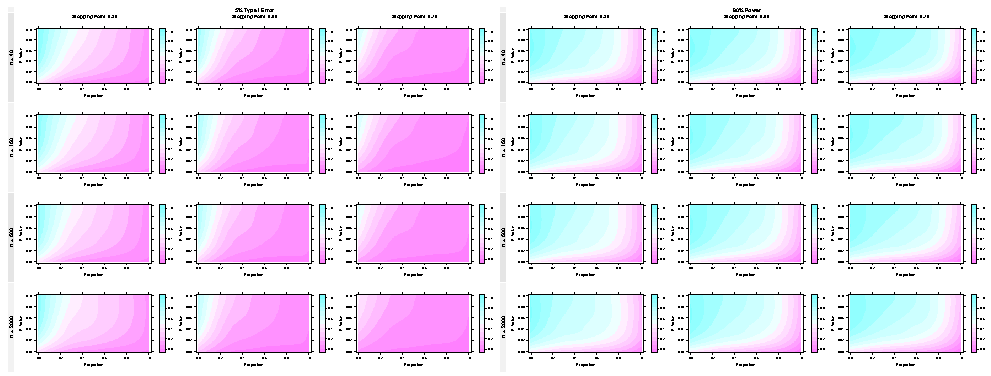
\includegraphics[width=\linewidth]{06_ManuscriptOutput_Figure1.pdf}
    \caption{\textit{Method Validation Results:}  Results reported as heatmaps showing the probability of meeting the defined p-value and proportion combination (blue representing more likely to meet the criteria, pink representing less likely) for various p-value (y axis) and proportion (x axis) threshold combinations.  The null (5\% Type I Error, left side) and alternative (80\% Power, right side) scenarios are presented with subplots faceted by information fraction at the interim look (0.25, 0.50, 0.75 from left to right) and maximum trial sample size (40, 160, 600, 2000 from top to bottom).}
    \label{fig:first}
  \end{minipage}\hfill%
\end{figure*}

\begin{figure*}[t]
  \begin{minipage}[t]{1\linewidth}
    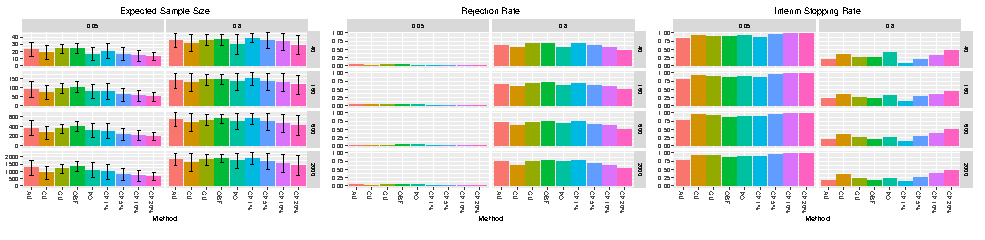
\includegraphics[width=\linewidth]{06_ManuscriptOutput_Figure2.pdf}
    \caption{\textit{Main Analysis Results:}  The left panel shows mean expected sample size (y axis) reported with error bars representing $\pm$ 1 SD for each interim monitoring method (x axis).  Graphing scale is relative to total sample size.  The middle panel shows rejection rate results, where rejection rate is defined as the proportion of simulated trials that reached trial completion and then rejected the null hypothesis.  Rejection rate (y axis) is reported for each interim monitoring method (x axis).  The right panel shows interim stopping rate results with interim stopping rate defined as the proportion of simulated trials that stopped early (y axis) reported for each interim monitoring method (x axis).  Subplots are faceted by power (5\% or 80\% from left to right) and total sample size (40, 160, 600, 2000 from top to bottom).}
    \label{fig:second}
  \end{minipage}\hfill%
\end{figure*}

\begin{figure*}[t]
  \begin{minipage}[t]{1\linewidth}
    
\includegraphics[width=\linewidth]{06_ManuscriptOutput_Figure3.pdf}
    \caption{\textit{Sensitivity Analysis Results:}  Results for a sensitivity analysis excluding the first interim stopping point (i.e. interim analyses are performed at 50\% and 75\% of the total planned sample).  The panels from left to right show mean expected sample size, rejection rate, and interim stopping rate.}
    \label{fig:third}
  \end{minipage}\hfill%
\end{figure*}


Before applying a specific calibration strategy (e.g., AU, CU, or GU), we first evaluated the general trends for sample sizes and information fractions across a grid of p-values and proportion of upstrapped samples less than or equal to that p-value. This allows for a validation of the general concept of upstrapping, which we present for both the null and alternative scenario.

Figure \ref{fig:first} displays heatmaps representing the probability of stopping the trial for futility based on the grid of threshold combinations, with different plots showing potential variation due to sample size, power, and the information fraction available at the interim look.  Results indicate that across sample sizes and information fractions the upstrap has a higher proportion of upstrapped samples meeting the criteria across different combinations in the null (5\% power) case rather than the alternative (80\% power) case. This can be thought of as interim monitoring for potential futility, where the higher proportions (i.e., greater pink shaded regions) in the null scenario indicate the upstrap is more likely to meet criteria for potential stopping.  These findings are encouraging and indicate that the method produces expected results when used to perform interim futility monitoring.  Additionally, results show similar trends across stopping points within a given sample size, as well as between sample sizes at the same stopping point.  Overall, the validation results provide evidence that upstrapping may be a possible approach for interim monitoring.


\subsection{Sequential Monitoring Results}

This section presents the results for the three proposed upstrap calibration approaches (AU, CU, and GU), two alpha-spending functions (PO and OBF), and four conditional power approaches (CP 1\%, CP 5\%, CP 10\%, and CP 20\%) when there are three interim looks at 0.25, 0.50, and 0.75 interim fractions of data under both null and the 80\% powered alternative scenarios. Each interim stopping rule starts with the traditional alpha-spending and conditional power results before introducing the results for the upstrap approaches.

Figure \ref{fig:second} present the expected sample size, rejection rates, and interim stopping rates, respectively. Table \ref{tab:main} presents the results for each interim monitoring strategy as the difference in rejection rate from a fixed sample (FS) design without interim monitoring and the ratio of the expected sample size to the fixed sample size for the null and alternative scenarios, respectively.  Also presented are the results of a sensitivity analysis removing the first scheduled interim analysis (numeric summaries shown in Table \ref{tab:sensitivity}). We additionally describe the general performance of the upstrap calibrations when under- or over-powered.  The specific numeric summaries of the under-  or over-powered scenarios are presented in the Supplementary Materials in Tables S1-S14. 


\subsubsection{Main Results}

The OBF method has type I error rates within 0.5\% of the FS design in the null scenario and reductions of approximately 2\% to power in the alternative scenario. The ESS across all sample sizes is about 65\% of the FS in the null when we expect to stop for futility, and around 92\% of the FS in the alternative when stopping for futility is sub-optimal. The PO method has similar type I error rates with even smaller ESS (around 50\% of FS under the null), but has a 10\% decrease in power relative to the FS design across all sample sizes.

The CP 1\% method has type I error rates around 1.5\% lower compared to FS, with simultaneous reductions in power of up to 5\%.  ESS is about 50\% of the FS in the null case and 95\% in the alternative case.  As the threshold value used in the CP methods increased from 1\% to 20\% the methods stops for futility progressively more often, leading to more pronounced decreases in both power and type I error rate relative to the FS design.  The most aggressive version of CP (CP 20\%) produced decreases in type I error rates of approximately 3\% and decreases in power of close to 25\%.  ESS is around 30\% of the FS in the null scenario and 70\% in the alternative scenario.  CP approaches with thresholds greater than 1\% showed undesirably large reductions in power compared to the FS design.

The CU upstrap calibration performs most similarly to the PO, albeit with a greater reduction in power at larger sample sizes of up to 18.5\%. The AU and GU upstrap calibrations have type I errors within 1\% of the FS design while needing only 58-62\% of the ESS. However, the AU power is 4.8-7.1\% lower with an ESS of 86-91\% of FS, and the GU difference in power increases from within 0.5\% of FS to 8.5\% lower as the sample size increases.

% conclusion, may move some to results if needed
CP designs are highly influenced by the percentage thresholds chosen but offer significant reductions in sample size, with CP 1\% performing best relative to other CP approaches.  The OBF is the most balanced with respect to type I error and power trade-offs, but the savings in ESS are minimal relative to the reductions with CP 1\%, AU, or GU upstrap calibrations for a futility only monitoring design. If decreasing the expected sample size is an important consideration, AU or GU may represent an acceptable trade-off considering it is about 5\% lower than OBF in all null scenarios.  AU and GU generally perform the comparably to CP 1\%, although CP 1\% performs moderately better in terms of ESS and power. Additionally, the AU requires no prior calibration, resulting in a low barrier to implementation.

\subsubsection{Results Excluding the 25\% Stopping Point}

Due to concerns that method performance might be inhibited by lack of sufficient data at particularly early stopping points, simulations dropping the earliest interim analysis (at 25\% of the full sample) were implemented.  Results from this sensitivity analysis are consistent with the main results findings overall, with small to moderate gains in operating characteristics across methods.  Without the possibility of stopping for futility at 25\% of the full sample ESS increased for all methods proportionally.  

While CP 1\% still performs best out of all four CP based methods, the decrease in power under the alternative is lessened compared to the main results findings, with power reductions of up to 1.8\% and 7.4\% for CP 1\% and CP 5\% respectively.  Type I error rate was consistent with previous results.  For ESS the difference between the four CP methods was narrower, ranging from about 55-65\% of FS under the null and 85-100\% under the alternative.

AU and CU both showed significant gains in power after excluding the first interim look, with power reductions between 1.2-6.8\% compared to FS for AU and 4.8-11.8\% for CU.  Type I error rate showed slight improvement, remaining within 1\% of FS for AU and within 1.3\% for CU.  Under the null scenario ESS was around 69\% of FS for AU and around 59\% for CU.  For the alternative ESS was approximately 95\% of FS for AU and 89\% for CU.  Results remain unchanged for GU since it's specific calibration approach already excludes the first interim stopping point.    

Excluding the first interim look does have a positive effect on performance of the upstrapping based designs.  Both AU and CU achieved improvements in power and type I error rate and higher ESS under the alternative scenario.  While ESS under the null scenario showed more modest results compared to the main findings, it was still significantly reduced compared to FS.  After excluding the first interim look the upstrapping designs were more comparable to both OBF, CP 5\%, and CP 1/%.  

\subsubsection{Results for Under- and Over-Powered Scenarios}

Simulations were also conducted to evaluate the performance of the interim monitoring methods if an underpowered (50\% power) or overpowered (95\% power) scenario were encountered when the design was calibrated assuming an effect size corresponding to 80\% power. These results are presented in the supplementary materials with figures and tables showing these scenarios for each of the operating characteristics. The underpowered scenario performs between the previously described null and alternative scenarios. The overpowered scenario has high rejection rates for most methods except PO which has lower power relative to the other approaches.

%\subsubsection{Performance of Upstrap Calibrations with Only a Single Interim Look}

%The upstrapping calibration performance when only conducting a single interim look differs from the design with three interim looks depending on the information fraction used. Since only one interim look is conducted, the observed type I error rate and power of each scenario are closer to that of the FS design. The ESS is minimized with a single look at 0.5. At a single 0.25 look, the ESS is higher due to having a less information to upstrap the remaining 75\% of the trial from. At a single 0.75 look, the ESS is also higher because the design only allows stopping after three-quarters of the study has been enrolled. The specific performance of these single interim looks are presented in the Supplementary Materials Tables S1-S14.

\section{Discussion}

There are numerous strategies for conducting interim monitoring within a clinical trial. In this paper we proposed the use of the non-parametric upstrap as a potential interim monitoring strategy and evaluated its potential performance across a range of calibration strategies. While we focus on the use of the upstrap in a binary outcome setting to facilitate comparison to existing alpha-spending and conditional power interim monitoring methods, the upstrap provides a flexible framework for statistical models with complexities that have not been fully addressed by existing methods. For example, the longitudinal ordinal logistic regression model used in the TREAT NOW clinical trial used an upstrapping approach \cite{R4, R9}.

While alpha-spending and conditional power approaches are well established methods for interim futility monitoring, both are limited by their parametric assumptions.  While these assumptions may be appropriate for many common data types and modeling strategies, there is a need for nonparametric alternatives to handle more the complex cases that often arise.  The upstrap shows great potential for filling this gap in available methodology, particularly since the results of this analysis found it comparable and in some cases even preferred in performance compared to traditional parametric designs in the simple case of a binary outcome.

The validation of the general performance of the upstrap across information fractions and sample sizes suggested promising performance for interim monitoring. Figure \ref{fig:first} demonstrated that the null scenario heat maps have far greater probability of meeting the given threshold combination, whereas the alternative scenario heat maps had far lower probabilities of meeting the thresholds and, potentially, stopping early for futility. 

In order to operationalize the upstrap for use in a trial, we proposed three different calibration strategies to evaluate the trial operating characteristics. These calibration strategies were then compared to existing Pocock (PO) and O'Brien-Fleming (OBF) alpha-spending approaches. The arbitrary (AU) approach was simplest in that the desired type I and II error levels can be used as the thresholds for the upstrap. The calibrated (CU) approach considers the specific scenario (e.g., sample size, null and alternative response, information fraction) to identify the thresholds and is more complicated. The groups-sequential (GU) approach to upstrapping used OBF p-value thresholds with only the proportion of upstrapped samples calibrated. However, none of the approaches explicitly accounted for the repeated looks at the data.

However, all upstrapping approaches do result in large reductions to the expected sample size (ESS) of the study relative to both PO and OBF alpha-spending approaches. Upstrapping approaches were generally more likely to stop a trial early compared to PO and OBF, as shown in Figure \ref{fig:second}.  Across all interim futility monitoring settings, the GU approach provided what may be considered as acceptable trade-offs in certain trial contexts considering the reductions in ESS relative to OBF of up to 8\% in null scenarios and 4\% in alternative scenarios, while having less inflation of the type I error rate than other calibration strategies. The CU approach was overly conservative for futility monitoring. Interestingly, the AU approach performed well in futility monitoring and could be an easy-to-implement approach if slightly lower power is acceptable or the maximum sample size could be increased.  Limiting interim analyses to occur later on in the trial (after accumulating a reasonable amount of data from which to make early stopping decisions) may be an effective way to further improve upstrapping approaches.


% Limitation paragraph 1
This research is an exploratory study of whether upstrapping may be a potential approach for interim monitoring, and there are potential limitations worth discussing.  First, many simplifying assumptions were made at both the simulation and modeling stages of our analysis.  We considered simulation settings based only on sample size, information fraction, and power.  All simulations assumed uniform subject accrual over time, and a constant treatment efficacy rate.  It may also be worth considering more complicated modeling strategies, potentially with covariate information included, to reflect a wider range of possible study design settings.

% Limitation paragraph 2
Calibration and application results showed a clear trade off between power and type I error rate for the general upstrapping method.  This is not unexpected, but is an important consideration when deciding on an interim monitoring method and choosing threshold values. In general, we considered several different approaches to threshold calibration and chose the best values based on power and type I error rate considerations.  However, this process could easily be extended to consider a wider variety of approaches or a more granular grid of potential threshold values.  Additional work is needed to develop calibration approaches for the upstrap which can better control the type I error rate while achieving the desired power. One possibility is to consider similarities with Bayesian interim monitoring using the predictive posterior probability (PPP), where the posterior probability may be analogous to the p-value and the PPP threshold analogous to our upstrapped proportion \cite{R10,R11,R12}.

%future work (efficacy monitoring)
Since the upstrap shows substantial promise in the futility monitoring context, one logical extension for future research is to also consider its use in efficacy monitoring.  Ideally such research would produce comparisons between upstrapping used for futility only monitoring, efficacy only monitoring, and combined interim  monitoring (allowing a trial to stop for either efficacy or futility depending on the results of the interim analysis).  Extending upstrapping to efficacy monitoring requires careful consideration of the method's relationship to conditional power analysis, and may perhaps require a more sophisticated approach to tuning parameter calibration.  Evaluating the upstrap's performance in efficacy monitoring would clearly present a more flexible and complex array of applications for the upstrap, and is worth exploring in order to continue expanding the scope of semi-parametric alternatives to traditional interim monitoring approaches.

Based on our simulation studies, the upstrap has potential to serve as a nonparametric approach to implementing interim analyses in clinical trials. In practice, the upstrap is flexible and could be generalized to a range of outcome types and study designs and is worth considering in future clinical trial designs for interim monitoring.


\section{Funding}
This work was supported by the United States Department of Defense (ID07200010-301-2) and The National Heart, Lung, and Blood Institute (K01 HL151754).

\section{Declaration of conflicting interests}
The Authors declare that there no conflicts of interest.

\section{Disclaimer}
The views expressed are those of the author(s) and do not reflect the official views or policy of the Department of Defense or its Components. The voluntary, fully informed consent of the subjects used in this research was obtained as required by 32 CFR 219 and DODI 3216.02\_AFI 40-402.

%%%%%%%%%%%%%%%%%%%%%%%%%%%%%%%%%%%%%%%%%%%%%%%%%%%%%%%% References

\begin{thebibliography}{99}
\bibitem[1]{R1}
DeMets, D. L., \& Lan, K. K. (1994). Interim analysis: the alpha spending function approach. \textit{Statistics in medicine, 13}(13-14), 1341–1356. https://doi.org/10.1002/sim.4780131308

\bibitem[2]{R2}
K.K. Gordon Lan, David M. Reboussin \& David L. DeMets (1994) Information and information fractions for design and sequential monitoring of clinical trials, Communications in Statistics - Theory and Methods, 23:2, 403-420, DOI: 10.1080/03610929408831263

\bibitem[3]{R3}
Jennison, C. and Turnbull, B. W. (1999). Group sequential methods with applications to clinical trials. CRC Press.

\bibitem[4]{R5}
O'Brien, P. C., \& Fleming, T. R. (1979). A multiple testing procedure for clinical trials. \textit{Biometrics, 35}(3), 549–556.

\bibitem[5]{R6}
Pocock, S. J. (1977). Group Sequential Methods in the Design and Analysis of Clinical Trials. \textit{Biometrika, 64}(2), 191–199. https://doi.org/10.2307/2335684

\bibitem[6]{R6b}
Pocock S. J. (1982). Interim analyses for randomized clinical trials: the group sequential approach. \textit{Biometrics, 38}(1), 153-62.

\bibitem[7]{R6c}
Proschan M. A., Lan K. G., Wittes J. T. (2006). Statistical monitoring of clinical trials: a unified approach. Springer Science \& Business Media..

\bibitem[8]{R4}
Kaizer, A. M., Wild, J., Lindsell, C. J., Rice, T. W., Self, W. H., Brown, S., Thompson, B. T., Hart, K. W., Smith, C., Pulia, M. S., Shapiro, N. I., \& Ginde, A. A. (2022). Trial of Early Antiviral Therapies during Non-hospitalized Outpatient Window (TREAT NOW) for COVID-19: a summary of the protocol and analysis plan for a decentralized randomized controlled trial. \textit{Trials, 23}(1), 273. https://doi.org/10.1186/s13063-022-06213-z

\bibitem[9]{R9}
Kaizer, A. M., Shapiro, N. I., Wild, J., Brown, S. M., Cwik, B. J., Hart, K. W., Jones, A. E., Pulia, M. S., Self, W. H., Smith, C., Smith, S. A., Ng, P. C., Thompson, B. T., Rice, T. W., Lindsell, C. J., \& Ginde, A. A. (2023). Lopinavir/ritonavir for treatment of non-hospitalized patients with COVID-19: a randomized clinical trial. \textit{International Journal of Infectious Diseases, 128}, 223-229.

\bibitem[10]{R7a}
Kundu, M.G., Samanta, S. \& Mondal, S. (2023). Review of calculation of conditional power, predictive power and probability of success in clinical trials with continuous, binary and time-to-event endpoints. \textit{Health Serv Outcomes Res Method}. https://doi.org/10.1007/s10742-023-00302-5

\bibitem[11]{R7b}
Saville BR, Detry MA, \& Viele K. (2023). Conditional Power: How Likely Is Trial Success?. \textit{JAMA}. 329(6):508–509. https://doi.org/10.1001/jama.2022.25080

\bibitem[12]{R7}
Crainiceanu, C. M., \& Crainiceanu, A. (2020). The upstrap. \textit{Biostatistics (Oxford, England), 21}(2), e164–e166. https://doi.org/10.1093/biostatistics/kxy054

\bibitem[13]{R8a}
Kundu MG (2022). LongCART: Recursive Partitioning for Longitudinal Data and Right Censored Data Using Baseline Covariates. R package version 3.2, <https://CRAN.R-project.org/package=LongCART>.

\bibitem[14]{R8b}
Zhang, Q., Freidlin, B., Korn, E. L., Halabi, S., Mandrekar, S., \& Dignam, J. J. (2017). Comparison of futility monitoring guidelines using completed phase III oncology trials. \textit{Clinical trials (London, England), 14}(1), 48–58. https://doi.org/10.1177/1740774516666502

\bibitem[15]{R8}
Alsouqi, A., Deger, S. M., Sahinoz, M., Mambungu, C., Clagett, A. R., Bian, A., Guide, A., Stewart, T. G., Pike, M., Robinson-Cohen, C., Crescenzi, R., Madhur, M. S., Harrison, D. G., \& Ikizler, T. A. (2022). Tissue Sodium in Patients With Early Stage Hypertension: A Randomized Controlled Trial. \textit{Journal of the American Heart Association, 11}(8), e022723. https://doi.org/10.1161/JAHA.121.022723

\bibitem[16]{R10}
Zabor E. C., Kaizer A. M., Garrett-Mayer E., \& Hobbs B. P. (2022) Optimal sequential predictive probability designs for early-phase oncology expansion cohorts. \textit{JCO Precision Oncology}(6), e2100390. https://doi.org/10.1200/PO.21.00390

\bibitem[17]{R11}
Dmitrienko A. \& Wang M. D. (2006) Bayesian predictive approach to interim monitoring in clinical trials. \textit{Statistics in medicine, 25}(13), 2178-95.

\bibitem[18]{R12}
Saville B. R., Connor J. T., Ayers G. D., \& Alvarez J. The utility of Bayesian predictive probabilities for interim monitoring of clinical trials. \textit{Clinical Trials, 11}(4), 485-93.

\end{thebibliography}


%%%%%%%%%%%%%%%%%%%%%%%%%%%%%%%%%%%%%%%%%%%%%%%%%%%%%%%% Results Table
\newpage
\onecolumn

\begin{sidewaystable}[]
\begin{tabular}{|l|l||C|C|C||C|C|C||C|C|C||C|C|C|}
\hline
 &  & \multicolumn{2}{c||}{\textit{\textbf{Null Scenario}}} & \multicolumn{2}{c|}{\textit{\textbf{Alternative Scenario}}}           \\ \hline \hline
\hline
\textbf{Method} & \textbf{N} & \multicolumn{1}{c||}{\textit{\textbf{Difference in TIE from Fixed Sample}}} & \multicolumn{1}{c|}{\textit{\textbf{Ratio of ESS to Fixed Sample}}} & \multicolumn{1}{c||}{\textit{\textbf{Difference in Power from Fixed Sample}}} & \multicolumn{1}{c|}{\textit{\textbf{Ratio of ESS to Fixed Sample}}}               \\ \hline \hline
CU                & 40   &   -0.007   &   0.48   &   -0.118   &   0.80   \\ \hline
CU                & 160  &   -0.011   &   0.46   &   -0.134   &   0.80   \\ \hline
CU                & 600  &   -0.015   &   0.45   &   -0.144   &   0.79   \\ \hline
CU                & 2000 &   -0.015   &   0.45   &   -0.185   &   0.79   \\ \hline \hline
AU                & 40   &    0.001   &   0.58   &   -0.048   &   0.90   \\ \hline
AU                & 160  &   -0.008   &   0.56   &   -0.071   &   0.86   \\ \hline
AU                & 600  &   -0.007   &   0.61   &   -0.061   &   0.89   \\ \hline
AU                & 2000 &   -0.005   &   0.62   &   -0.068   &   0.91   \\ \hline \hline
GU                & 40   &    0.002   &   0.60   &    0.005   &   0.90   \\ \hline
GU                & 160  &    0.000   &   0.61   &   -0.031   &   0.91   \\ \hline
GU                & 600  &   -0.006   &   0.59   &   -0.073   &   0.89   \\ \hline
GU                & 2000 &   -0.008   &   0.59   &   -0.085   &   0.90   \\ \hline \hline
OBF               & 40   &    0.002   &   0.62   &    0.003   &   0.90   \\ \hline
OBF               & 160  &    0.002   &   0.64   &   -0.016   &   0.92   \\ \hline
OBF               & 600  &    0.002   &   0.66   &   -0.032   &   0.93   \\ \hline
OBF               & 2000 &   -0.005   &   0.67   &   -0.028   &   0.94   \\ \hline \hline
PO                & 40   &   -0.006   &   0.42   &   -0.122   &   0.75   \\ \hline
PO                & 160  &   -0.002   &   0.49   &   -0.092   &   0.82   \\ \hline
PO                & 600  &   -0.002   &   0.53   &   -0.094   &   0.84   \\ \hline
PO                & 2000 &   -0.001   &   0.54   &   -0.083   &   0.87   \\ \hline \hline
CP 1\%            & 40   &   -0.009   &   0.52   &   -0.004   &   0.98   \\ \hline
CP 1\%            & 160  &   -0.023   &   0.50   &   -0.025   &   0.92   \\ \hline
CP 1\%            & 600  &   -0.014   &   0.50   &   -0.030   &   0.93   \\ \hline
CP 1\%            & 2000 &   -0.019   &   0.49   &   -0.049   &   0.93   \\ \hline \hline
CP 5\%            & 40   &   -0.017   &   0.42   &   -0.052   &   0.90   \\ \hline
CP 5\%            & 160  &   -0.028   &   0.39   &   -0.097   &   0.83   \\ \hline
CP 5\%            & 600  &   -0.018   &   0.38   &   -0.114   &   0.83   \\ \hline
CP 5\%            & 2000 &   -0.025   &   0.39   &   -0.124   &   0.85   \\ \hline \hline
CP 10\%           & 40   &   -0.023   &   0.38   &   -0.122   &   0.85   \\ \hline
CP 10\%           & 160  &   -0.030   &   0.34   &   -0.127   &   0.80   \\ \hline
CP 10\%           & 600  &   -0.024   &   0.34   &   -0.161   &   0.78   \\ \hline
CP 10\%           & 2000 &   -0.031   &   0.34   &   -0.205   &   0.78   \\ \hline \hline
CP 20\%           & 40   &   -0.025   &   0.32   &   -0.215   &   0.72   \\ \hline
CP 20\%           & 160  &   -0.035   &   0.31   &   -0.210   &   0.72   \\ \hline
CP 20\%           & 600  &   -0.026   &   0.31   &   -0.272   &   0.69   \\ \hline
CP 20\%           & 2000 &   -0.035   &   0.31   &   -0.298   &   0.71   \\ \hline \end{tabular}
\caption{\textit{Main results} from alternative and null scenario simulations for the performance of the interim analysis calibration method relative to the fixed sample design. CU is the calibrated upstrap, AU is the arbitrary upstrap, GU is the group-sequential upstrap, OBF is the O'Brien-Fleming alpha-spending function, PO is the Pocok alpha-spending function, CP is the conditional power method.}
\label{tab:main}
\end{sidewaystable}

\begin{sidewaystable}[]
\begin{tabular}{|l|l||C|C|C||C|C|C||C|C|C||C|C|C|}
\hline
 &  & \multicolumn{2}{c||}{\textit{\textbf{Null Scenario}}} & \multicolumn{2}{c|}{\textit{\textbf{Alternative Scenario}}}           \\ \hline \hline
\hline
\textbf{Method} & \textbf{N} & \multicolumn{1}{c||}{\textit{\textbf{Difference in TIE from Fixed Sample}}} & \multicolumn{1}{c|}{\textit{\textbf{Ratio of ESS to Fixed Sample}}} & \multicolumn{1}{c||}{\textit{\textbf{Difference in Power from Fixed Sample}}} & \multicolumn{1}{c|}{\textit{\textbf{Ratio of ESS to Fixed Sample}}}               \\ \hline \hline
0.50-0.75 CU                & 40   &   -0.002   &   0.60   &   -0.048   &   0.90   \\ \hline
0.50-0.75 CU                & 160  &   -0.007   &   0.59   &   -0.064   &   0.89   \\ \hline
0.50-0.75 CU                & 600  &   -0.011   &   0.58   &   -0.077   &   0.88   \\ \hline
0.50-0.75 CU                & 2000 &   -0.013   &   0.58   &   -0.118   &   0.88   \\ \hline \hline
0.50-0.75 AU                & 40   &    0.004   &   0.68   &   -0.012   &   0.95   \\ \hline
0.50-0.75 AU                & 160  &   -0.004   &   0.68   &   -0.019   &   0.94   \\ \hline
0.50-0.75 AU                & 600  &   -0.006   &   0.69   &   -0.023   &   0.94   \\ \hline
0.50-0.75 AU                & 2000 &   -0.005   &   0.70   &   -0.068   &   0.95   \\ \hline \hline
0.50-0.75 GU                & 40   &    0.002   &   0.60   &    0.005   &   0.90   \\ \hline
0.50-0.75 GU                & 160  &    0.000   &   0.61   &   -0.031   &   0.91   \\ \hline
0.50-0.75 GU                & 600  &   -0.006   &   0.59   &   -0.073   &   0.89   \\ \hline
0.50-0.75 GU                & 2000 &   -0.008   &   0.59   &   -0.085   &   0.90   \\ \hline \hline
0.50-0.75 CP 1\%            & 40   &   -0.009   &   0.65   &    0.002   &   1.00   \\ \hline
0.50-0.75 CP 1\%            & 160  &   -0.022   &   0.63   &   -0.007   &   0.96   \\ \hline
0.50-0.75 CP 1\%            & 600  &   -0.014   &   0.63   &   -0.005   &   0.96   \\ \hline
0.50-0.75 CP 1\%            & 2000 &   -0.019   &   0.62   &   -0.018   &   0.97   \\ \hline \hline
0.50-0.75 CP 5\%            & 40   &   -0.013   &   0.58   &   -0.006   &   0.98   \\ \hline
0.50-0.75 CP 5\%            & 160  &   -0.023   &   0.58   &   -0.031   &   0.92   \\ \hline
0.50-0.75 CP 5\%            & 600  &   -0.017   &   0.56   &   -0.056   &   0.91   \\ \hline
0.50-0.75 CP 5\%            & 2000 &   -0.024   &   0.56   &   -0.074   &   0.92   \\ \hline \hline
0.50-0.75 CP 10\%           & 40   &   -0.016   &   0.55   &   -0.078   &   0.92   \\ \hline
0.50-0.75 CP 10\%           & 160  &   -0.028   &   0.54   &   -0.060   &   0.90   \\ \hline
0.50-0.75 CP 10\%           & 600  &   -0.022   &   0.54   &   -0.097   &   0.88   \\ \hline
0.50-0.75 CP 10\%           & 2000 &   -0.029   &   0.54   &   -0.125   &   0.88   \\ \hline \hline
0.50-0.75 CP 20\%           & 40   &   -0.020   &   0.55   &   -0.115   &   0.88   \\ \hline
0.50-0.75 CP 20\%           & 160  &   -0.033   &   0.52   &   -0.139   &   0.84   \\ \hline
0.50-0.75 CP 20\%           & 600  &   -0.026   &   0.52   &   -0.178   &   0.83   \\ \hline
0.50-0.75 CP 20\%           & 2000 &   -0.033   &   0.52   &   -0.222   &   0.83   \\ \hline \end{tabular}
\caption{\textit{Sensitivity analysis results} from alternative and null scenario simulations for the performance of the interim analysis calibration method, excluding the first interim stopping point, relative to the fixed sample design. CU is the calibrated upstrap, AU is the arbitrary upstrap, GU is the group-sequential upstrap, OBF is the O'Brien-Fleming alpha-spending function, PO is the Pocok alpha-spending function, CP is the conditional power method.}
\label{tab:sensitivity}
\end{sidewaystable}

\end{document}